\documentclass{cubeamer}

\title{Introdução ao Arduino}
\subtitle{Workshop de Arduino - \textbf{rascimatec}}
\author[João Vítor Silva Mendes]{João Vítor Silva Mendes.}
\date{\today} % or whatever the date you are presenting in is
\institute[SENAI CIMATEC]{SENAI CIMATEC - IEEE ROBOTICS AND AUTOMATION SOCIETY}
% \copyrightnotice{Published by the American Institute of Aeronautics and Astronautics, Inc., with permission}
\usepackage{ragged2e}
\begin{document}

\maketitle

\cutoc

\section{Introdução}

\begin{frame}{RAS CIMATEC}
    \begin{columns}

        \begin{column}{0.4\textwidth}
            \begin{itemize}
                \item Quem somos?
                \item O que fazemos?
                \item Para quem?
            \end{itemize}
        \end{column}

        \begin{column}{0.6\textwidth}
            \begin{figure}
                \centering
                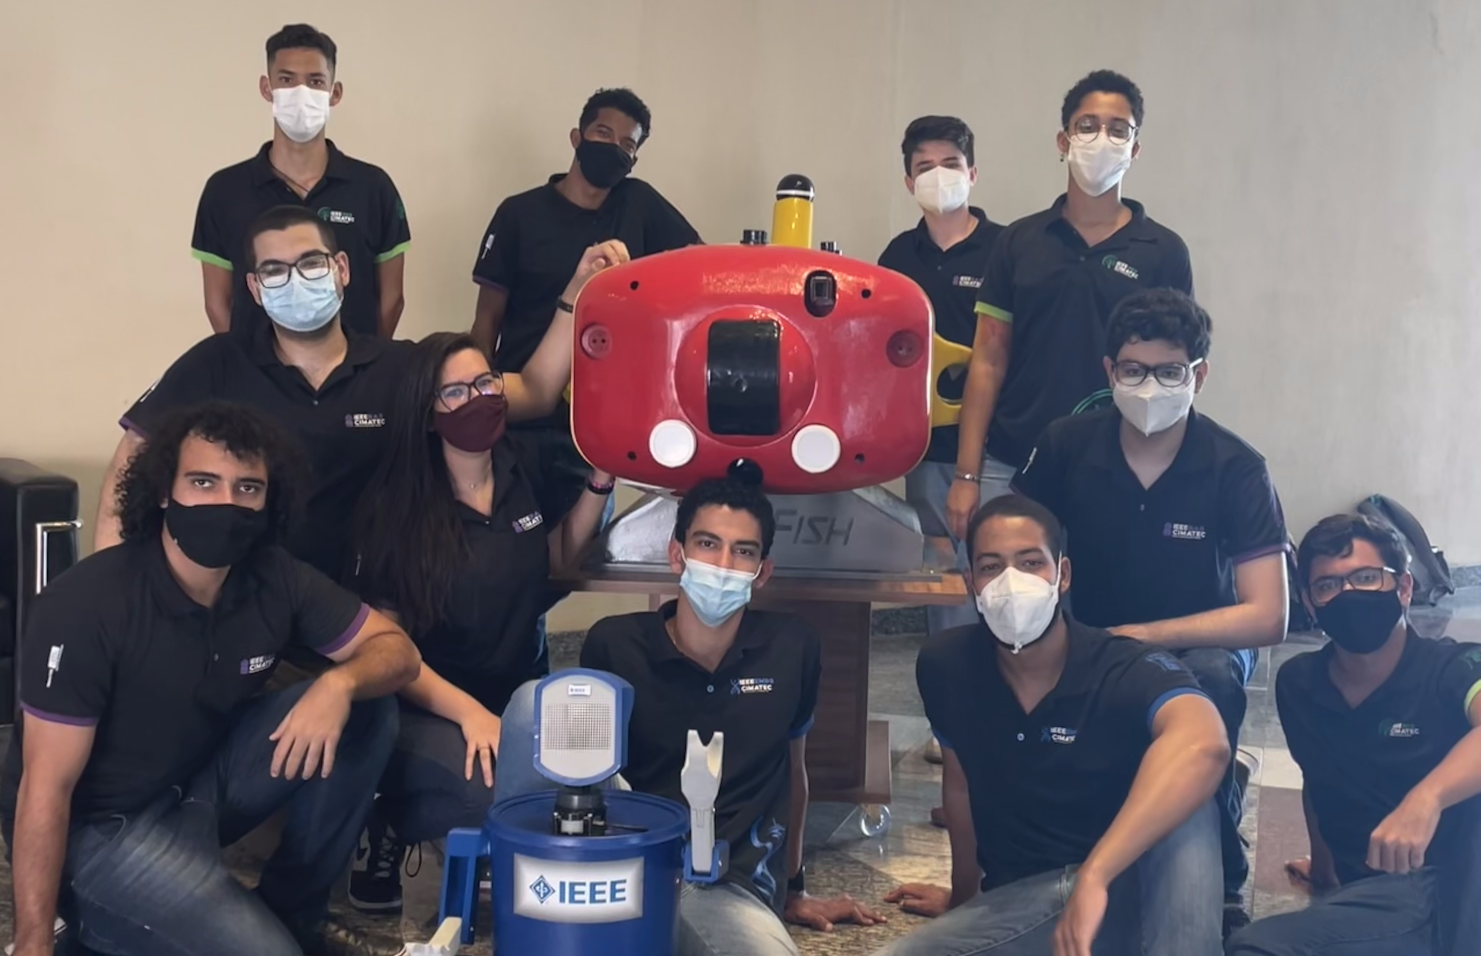
\includegraphics[height = 0.6\textheight]{img/team2.png}
                % \caption{Fancy Thing from \textit{Source et al.}}
            \end{figure}
        \end{column}

    \end{columns}
\end{frame}

\begin{frame}{Apresentação do mediador}
    \begin{columns}
        \centering
        \begin{column}{0.3\textwidth}
            \begin{figure}
                \centering
                
\includegraphics[height = 0.5\textheight]{img/mediador.png}
                \caption[]{Vítor Mendes}
            \end{figure}
        \end{column}
        \centering
        \begin{column}{0.5\textwidth}
            \footnotesize
            \justifying
            Estudante de Engenharia Elétrica no SENAI CIMATEC, atual presidente da RAS CIMATEC. Como bolsista de IC PIBIC(FAPESB), faz parte do Grupo de Pesquisa Integração Digital para Manufatura Avançada, atuando no projeto que visa automatizar o monitoramento de linhas de produção de petróleo(PRH 27.1). Atuou na RAS como secretário na gestão de 2021, na área de gerenciamento de projetos e produção de eventos, além de fazer parte da equipe de desenvolvimento do MapVision.

        \end{column}
    \end{columns}
\end{frame}

\begin{frame}{Apresentação do curso}
    \begin{columns}
        \centering
        \begin{column}{0.4\textwidth}
            \textbf{1° Dia} \\
            \small
            Introdução à Plataforma;\\
            Como programar um microcontrolador;\\
            Demonstração do Projeto 1\\

        \end{column}
        \begin{column}{0.5\textwidth}
            \textbf{2° Dia} \\
            \small
            Conceitos básicos de eletrônica;\\
            Como programar um microcontrolador;\\
            P1 - Sistema de medição de distância por ultrassom;\\
            P2 - Sistema de acionamento de motores;\\
        \end{column}
    \end{columns}
\end{frame}

\begin{frame}{Apresentação do curso}
    \begin{columns}
        \centering
        \begin{column}{0.5\textwidth}
            \textbf{3° Dia} \\
            \small
            Construindo meu primeiro robô.
        \end{column}
    \end{columns}
\end{frame}

\begin{frame}{O que é Arduino}
    \begin{columns}

        \begin{column}{0.5\textwidth}
            \begin{itemize}
                \item O que é?
                \item Missão
                \item Sua importância
            \end{itemize}
        \end{column}
    
        \centering
        \begin{column}{0.4\textwidth}
            \begin{figure}
                \centering
                
\includegraphics[height = 0.6\textheight]{img/arduino.png}
            \end{figure}
        \end{column}
        \centering

    \end{columns}
\end{frame}

\begin{frame}{Placas de desenvolvimento}


    \begin{figure}
        \centering
        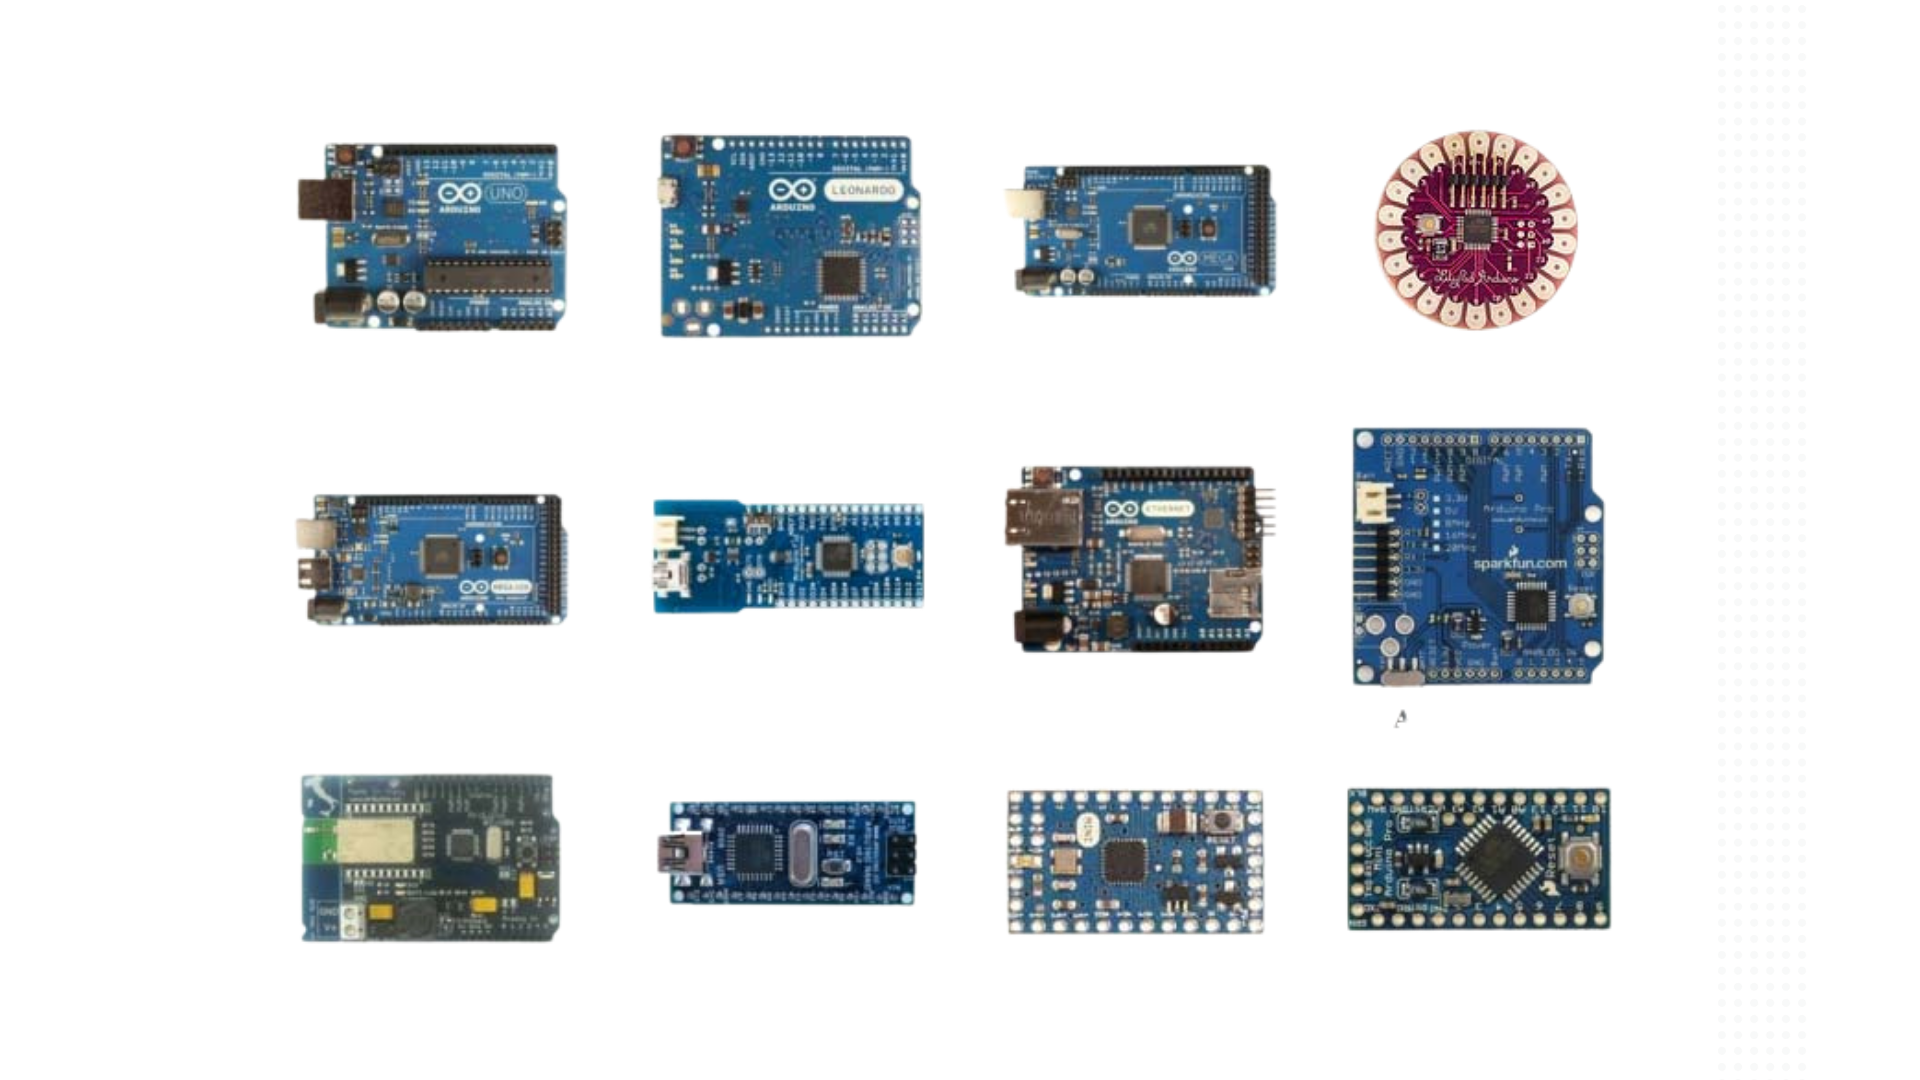
\includegraphics[height = 0.9\textheight]{img/placas.png}
    \end{figure}


\end{frame}

\begin{frame}{Arduino UNO}


    \begin{figure}
        \centering
        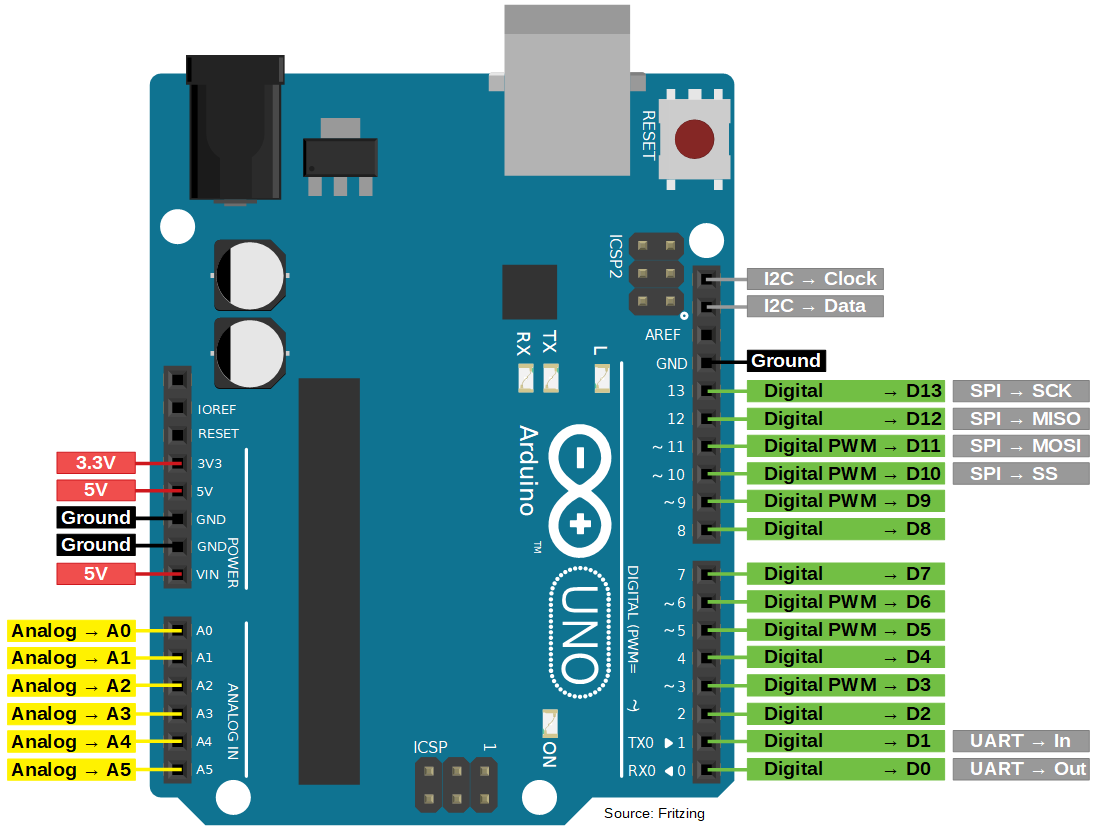
\includegraphics[height = 0.7\textheight]{img/uno.png}
    \end{figure}


\end{frame}

\section{O que é Arduino?}

\begin{frame}{Make your presentation interactive}
    \begin{cublock}[What about a question to the audience?]
        \begin{overlayarea}{\textwidth}{\baselineskip}
            \only<2->{Followed by the answer.}
        \end{overlayarea}
    \end{cublock}
\end{frame}

% Q&A
\begin{frame}[standout]
    \Huge\textsc{Thank You}
    
    \vfill
    
    \LARGE\textsc{Questions?}
\end{frame}

\appendix

\begin{frame}{Backup slides go here}
    
\end{frame}

\end{document}
